\subsection{Hyperledger Composer}
        Hyperledger Composer ist ein Framework für das Entwickeln von Blockchain-Netzwerken und dient vornehmlich als Abstraktion des Hyperledger Fabric Frameworks. 
        \medskip\\
        Fabric bietet die Möglichkeit Private- oder Consortium-Blockchainnetzwerke zu entwickeln und zu betreiben, wobei eigens konfigurierbare 
        \medskip\\
        \noindent Für die Entwicklung der Transaktionslogik von Business Networks wird die Sprache JavaScript verwendet. 
        Zusätzlich werden domainspezifische Sprachen für die Modellierung der Akteure im Netzwerk, sowie der Zugriffskontrolle und Anfragen and die Blockchcain eingesetzt.
        Als Datenbank kann LevelDB oder CouchCB verwendet werden. 
        
        \noindent Für den Prototypen relevante Eigenschaften des Hyperledger Composer Frameworks:
        \begin{itemize}[noitemsep]
            \item Ein Blockchain-Netzwerk wird im Kontext des Frameworks als ,,Business Network`` bezeichnet. 
            \item Ein Business Network besteht aus Assets, Participants, Transactions, \gls{acl}, Events (optional) und Queries (optional).
                \begin{itemize}[noitemsep]
                    \item Assets: Güter, die auf der Blockchain gespeichert sind.
                    \item Participants: Teilnehmer des Netzwerkes.
                    \item Transactions: Funktionen, die ausgeführt werden können, können Smart Contracts (Transaction Processor Functions) auslösen, welche beliebige Aktionen ausfüren können. 
                    \item Access Control Rules: legen fest, welche Teilnehmer welche Aktionen im Netzwerk ausüben dürfen. 
                        Zu vergebende Berechtigungen (CRUD
                        \!\footnote{Create, Read, Update, Delete}
                        ) beschränken sich auf Assets und Transactions und werden sequentiell in geordneter Reihenfolge ausgewertet. 
                \end{itemize}
            \item Metadaten wie Dependencies und Versionsnummern werden in einer separaten Datei (\colorbox{light-gray}{\lstinline|package.json|}) abgelegt.
            \item bei der Ausführung einer Transaktion kann gleichzeitig optional ein Smart Contract ausgeführt werden
            \item Historian registry: The historian is a specialised registry which records successful transactions, including the participants and identities that submitted them. 
            The historian stores transactions as HistorianRecord assets, which are defined in the Hyperledger Composer system namespace.
        \end{itemize}
        
        \begin{figure}[H]
    		\centering
    		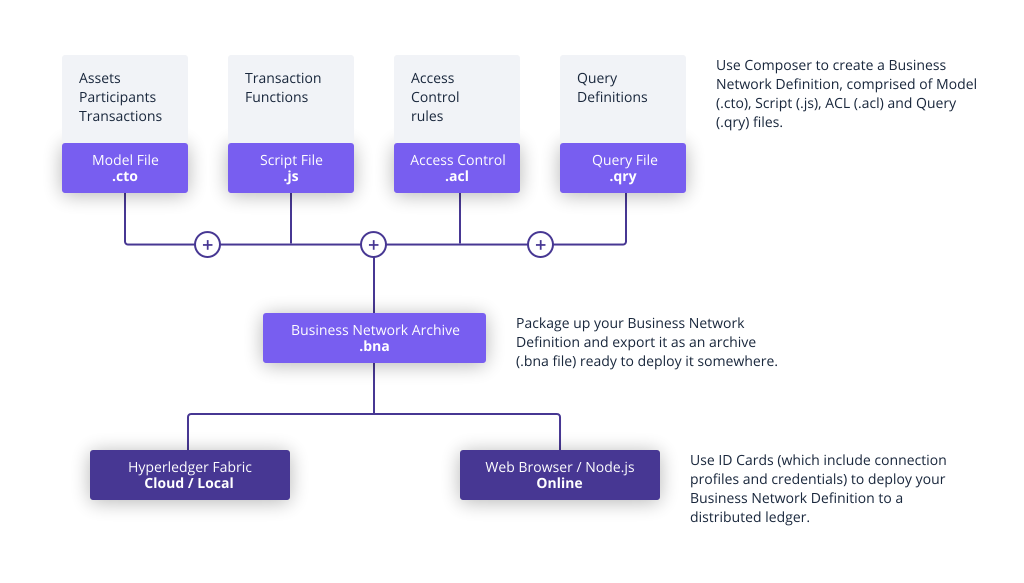
\includegraphics[width=\textwidth]{graphics/Composer-Diagram.png}
    		\caption[Bestandteile einer Hyperledger Composer-Applikation]{Bestandteile einer Hyperledger Composer-Applikation\cite{ComposerDocs}}
    		\label{fig:composer_arch}
    	\end{figure}
        
        \begin{itemize}[noitemsep]
            \item Möglichkeit eine REST-\gls{api} pro Business Network Card mit folgenden Features zu generieren
                \begin{itemize}[noitemsep]
                    \item Nutzung von API-Keys für die Sicherung der REST-\gls{api}
                    \item Authentifizierung via Passport auf Linux-Maschinen
                    \item ,,Explorer Test Interface``, welches automatisch generiert wird und essentiell eine Dokumentation der \gls{api} darstellt mit der zusätzlichen Möglichkeit die \gls{api}-Calls zu testen.
                    \item Key für dynamisches Logging
                    \item Event Publication via WebSocket
                    \item \gls{tls} und HTTPS für die \gls{api}
                \end{itemize}
            \item Bietet die Möglichkeit eine simple Anuglar-App zu generieren, welche letztendlich nur eine GUI-Maske für die \gls{api}-Methoden ist.
            \item Actors im Netzwerk (Peers, Orderers, Client Applications etc. haben eine digitale Identität, welche sich in einem X.509 digitalem Zeritifikat befindet.
                Die Zertifikate sind letztendlich ausschlaggebend für die Zugriffskontrolle und den Rechten, die eine Entität in dem Netzwerk erhält. 
                Zusätzlich können weitere Attribute, die zu einer Identät gehören genutzt werden (wie bspw. Organisiation, Rolle, etc.), welche eine Rolle bei der Bestimmung, welche Rechte diese Entität erhalten soll, spielen können.
            \item Zertifikate kommen von einer vertrausenswürdigen Autortität, dem \gls{msp}. 
                Gleicht einer PKI mit digitalen Zertifikaten, public/\-private Keys, CA und CRL
            \item öffentliche und private Kanäle: Nachrichtenwege, um Privatsphäre von Transaktionen und Vertraulichkeit zu gewährleisten.
                Private Kanäle sind nur für bestimmte Netzwerkmitglieder sichtbar, denen der Channel freigegeben wurde.
            \item Ordering Service: ein oder mehrere Knoten, die Transaktionen in einem Block ordnen
            \item Ledger: Blockchain + World State
            \item Deployable: Business Network Archive (bna)
            \item Historian: registry which records successful transactions, including the participants and identities that submitted them
        \end{itemize}
        
        \begin{itemize}[noitemsep]
            \item Single Organization 
            \item Membership Provider Service
        \end{itemize}
    
